\documentclass[
	article,
	11pt,
	twoside,
	a4paper,
	english,
	brazil,
	sumario=tradicional
	]{abntex2}

\usepackage{helvet} 
\usepackage[T1]{fontenc}		
\usepackage[utf8]{inputenc}	
\usepackage{indentfirst}
\usepackage{nomencl}
\usepackage{color}
\usepackage{graphicx}
\usepackage[export]{adjustbox}
\usepackage{microtype}
\usepackage{float}
\usepackage{pdfpages}
\usepackage{scalefnt}
\usepackage{authblk}
\usepackage{multicol}
\usepackage{amsmath}
\usepackage{wrapfig}
\usepackage{amssymb}
\usepackage{tikz}
\usetikzlibrary{shapes.geometric,fit}
\usepackage{nameref}
\usepackage{blindtext}
\usepackage{hyperref}

\linespread{1.5}

\renewcommand\Authands{ e }
\renewcommand{\familydefault}{\sfdefault}

\setlrmarginsandblock{4cm}{4cm}{*}
\setulmarginsandblock{4cm}{4cm}{*}
\checkandfixthelayout

%\usepackage[brazilian,hyperpageref]{backref}	 % 
\usepackage[alf]{abntex2cite}

\titulo{2ª Prova de Fundamentos Matemáticos para Computação} 
\author[*]{Ítalo Epifânio de Lima e Silva}
\affil[*]{Universidade Federal do Rio Grande do Norte, UFRN}

\local{Natal, RN}
\data{2019}

\definecolor{blue}{RGB}{41,5,195}

\makeatletter
\hypersetup{
     	%pagebackref=true,
		pdftitle={\@title}, 
		pdfauthor={\@author},
    	pdfsubject={Modelo de artigo científico com abnTeX2},
	    pdfcreator={LaTeX with abnTeX2},
		pdfkeywords={abnt}{latex}{abntex}{abntex2}{atigo científico}, 
		colorlinks=true,       		% false: boxed links; true: colored links
    	linkcolor=blue,          	% color of internal links
    	citecolor=blue,        		% color of links to bibliography
    	filecolor=magenta,      		% color of file links
		urlcolor=blue,
		bookmarksdepth=4
}
\makeatother

\makeindex


\setlrmarginsandblock{3cm}{3cm}{*}
\setulmarginsandblock{3cm}{3cm}{*}
\checkandfixthelayout

\setlength{\parindent}{1.3cm}

\setlength{\parskip}{0.2cm}  

\SingleSpacing

\begin{document}

\frenchspacing 

\maketitle

\textual

\section*{Questão 01}
\addcontentsline{toc}{section}{Questão 01}
\noindent
\subsection*{01 - Sejam 
$ f \colon \mathbb{R} \to \mathbb{R} $ 
e 
$ g \colon \mathbb{R} \to \mathbb{R} $ 
duas funções injetivas. A função  definida por 
$ h(x) = f (x) + g(x) $
é injetiva? (Aqui $+$ denota a usual adição entre números reais)
}

A função $ h(x) $ não é injetiva. Mostremos um contra-exemplo:

Seja $ g $ e $ f $ definidas por $ g(x) = -x $ e $ f(x) = x $. 

Note que ambas são \hyperlink{injetivas}{injetivas}.

Dessa forma $ h(x) = -x + x $ e, portanto, $ h(x) = 0 $

Uma função constante e não injetiva, pois existem dois (nesse caso todos) elementos do domínio de $ h $ que apontam para mais de um elemento do contradomínio.

\begin{comment}

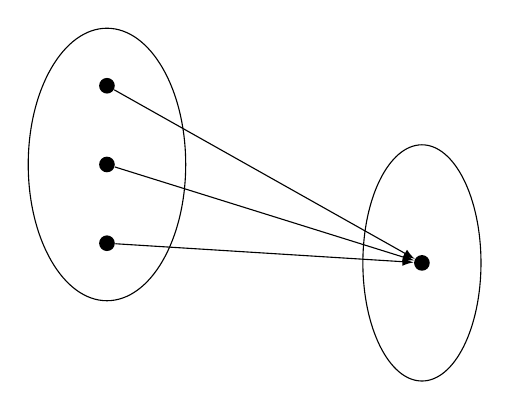
\begin{tikzpicture}
%put some nodes on the left
\foreach \x in {1,2,3}{
	\node[fill,circle,inner sep=2pt] (d\x) at (0,\x) {};
}
\node[fit=(d1) (d2) (d3),ellipse,draw,minimum width=2cm, minimum height = 3cm] {}; 

%put some nodes on the right
\foreach \x[count=\xi] in {0.75}{
	\node[fill,circle,inner sep=2pt] (c\xi) at (4,\x) {};
}
\node[fit=(c1) (c1) (c1) ,ellipse,draw,minimum width=1.5cm, minimum height = 3cm] {};
\draw[-latex] (d1) -- (c1);
\draw[-latex] (d2) -- (c1);
\draw[-latex] (d3) -- (c1);
\end{tikzpicture}

\end{comment}

\subsection*{Mostrando a injetividade de $ f $ e $ g $:}

Demostrando que $ f $ e $ g $ são \hypertarget{injetivas}{injetivas}:

Seja $ x, y \in \mathbb{R} $ tal que $ f(x) = f(y) $, logo $ x = y $, portanto $ f $ é injetiva.

Seja $ w, z \in \mathbb{R} $ tal que $ g(w) = g(z) $, logo $ -z = -w $ e $ z = w $, portanto $ g $ é injetiva.



\newpage
\section*{Questão 02}
\addcontentsline{toc}{section}{Questão 02}
\noindent
\subsection*{
02 - Sejam 
$ f \colon A \to B $ e $ g \colon B \to A $ 
funções totais \hypertarget{h1}{(H1)}, e tais que 
$ f \circ g = Id_{B} $ 
\hypertarget{h2}{(H2)}, mas 
$ g \circ f \neq IdA $ \hypertarget{h3}{(H3)}.
}



2a) Demonstre que a função f não pode ser injetiva.

2b) Demonstre que a função g não pode ser sobrejetiva.


\subsubsection*{2a)} 

Suponha que $ f $ é injetora. 

Por (H3) existem $ (a,a') \in A $, com $ a \neq a' $ e $ (a,a') \in g \circ f $

Pela definição de composição, existe $ b \in B $ tal que $ (a,b) \in f $ e $ (b,a') \in g $

Por (H2), $ (f \circ g)(b) = Id_{B}(b)$, pela definição de identidade e composição $ f(g(b)) = b $

Note que $ g(b) =  a' $, logo $ f(a') = b $
 
Note que, $ f(a) = b $, logo $ f(a) = f(a') $

Como $ f $ é injetiva, então $ a = a' $, o que contradiz (H3), portanto $ f $ não é injetiva.

\subsubsection*{2b)}

Por 2a) f não é injetiva e portanto, existem $ a, a' \in A $ tal que $ f(a) = f(a') $ e $ a \neq a' $

Suponha que $ g $ é sobrejetiva

Pela definição de sobrejetividade, existem $ (b, b') \in B $ tal que $ g(b) = a $ e $ g(b') = a' $

Note que $ b \neq b' $, por $ g $ ser função total

Note que $ (f \circ g)(b) $, pela definição de composição $ f(g(b)) $ e como $ g(b) = a $, então $ f(g(b)) = f(a) $ (I)

Note que $ (f \circ g)(b') $, pela definição de composição $ f(g(b')) $ e como $ g(b') = a' $, então $ f(g(b')) = f(a') $ (II)

Por (H2) $ (f \circ g)(b) = Id_{B}(b) $, pela definição de identidade e composição $ f(g(b)) = b $ e por (I) $ f(g(b)) = b = f(a) $

Por (H2) $ (f \circ g)(b') = Id_{B}(b') $, pela definição de identidade e composição $ f(g(b')) = b' $ e por (I) $ f(g(b')) = b' = f(a') $

Como $ f(a) = b $ e $ f(a') = b' $, então $ b = b' $, o que contradiz $ g $ ser função total, portanto, $ g $ não é sobrejetiva.



\end{document}